\section{Referencia de la Estructura cola\-Err}
\label{structcolaErr}\index{colaErr@{colaErr}}
Cola de errores.  


{\tt \#include $<$colaerr.h$>$}

Diagrama de colaboraci\'{o}n para cola\-Err:\begin{figure}[H]
\begin{center}
\leavevmode
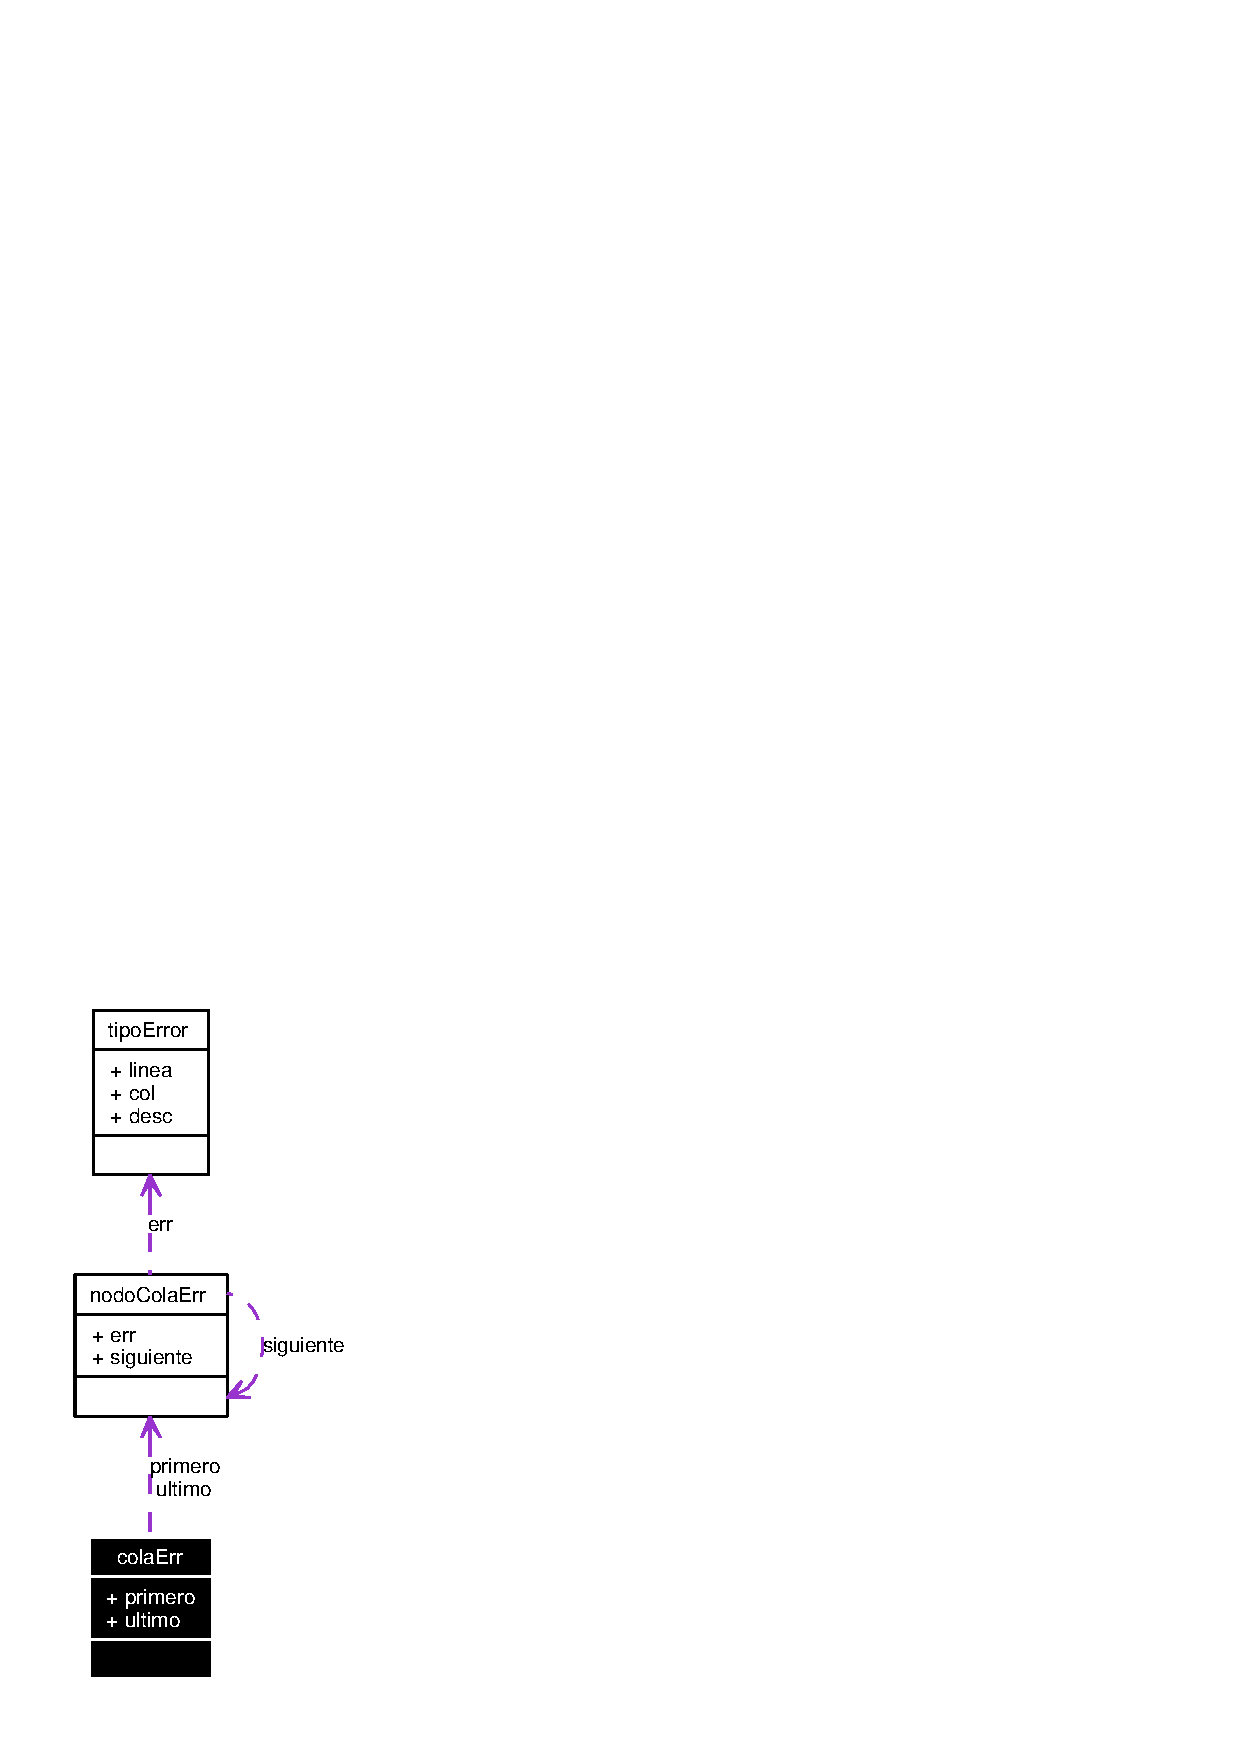
\includegraphics[width=83pt]{structcolaErr__coll__graph}
\end{center}
\end{figure}
\subsection*{Atributos p\'{u}blicos}
\begin{CompactItemize}
\item 
{\bf nodo\-Cola\-Err} $\ast$ {\bf primero}
\item 
{\bf nodo\-Cola\-Err} $\ast$ {\bf ultimo}
\end{CompactItemize}


\subsection{Descripci\'{o}n detallada}
Cola de errores. 



Definici\'{o}n en la l\'{\i}nea 39 del archivo colaerr.h.

\subsection{Documentaci\'{o}n de los datos miembro}
\index{colaErr@{cola\-Err}!primero@{primero}}
\index{primero@{primero}!colaErr@{cola\-Err}}
\subsubsection{\setlength{\rightskip}{0pt plus 5cm}{\bf nodo\-Cola\-Err}$\ast$ {\bf cola\-Err::primero}}\label{structcolaErr_o0}




Definici\'{o}n en la l\'{\i}nea 40 del archivo colaerr.h.

Referenciado por encolar\-Error(), escribir\-Error\-Log\-XML(), y sacar\-Error().\index{colaErr@{cola\-Err}!ultimo@{ultimo}}
\index{ultimo@{ultimo}!colaErr@{cola\-Err}}
\subsubsection{\setlength{\rightskip}{0pt plus 5cm}{\bf nodo\-Cola\-Err}$\ast$ {\bf cola\-Err::ultimo}}\label{structcolaErr_o1}




Definici\'{o}n en la l\'{\i}nea 41 del archivo colaerr.h.

Referenciado por encolar\-Error(), y sacar\-Error().

La documentaci\'{o}n para esta estructura fu\'{e} generada a partir del siguiente archivo:\begin{CompactItemize}
\item 
/media/docs/progra/c++/compiladores1/proy2/godzilla/src/{\bf colaerr.h}\end{CompactItemize}
